\section{实验记录及结果展示}

\subsection{实验记录}
主要是通过调整奖励、学习率、模型以及Q值计算公式等来获得更高的参数。
\begin{figure}[H]
    \centering
    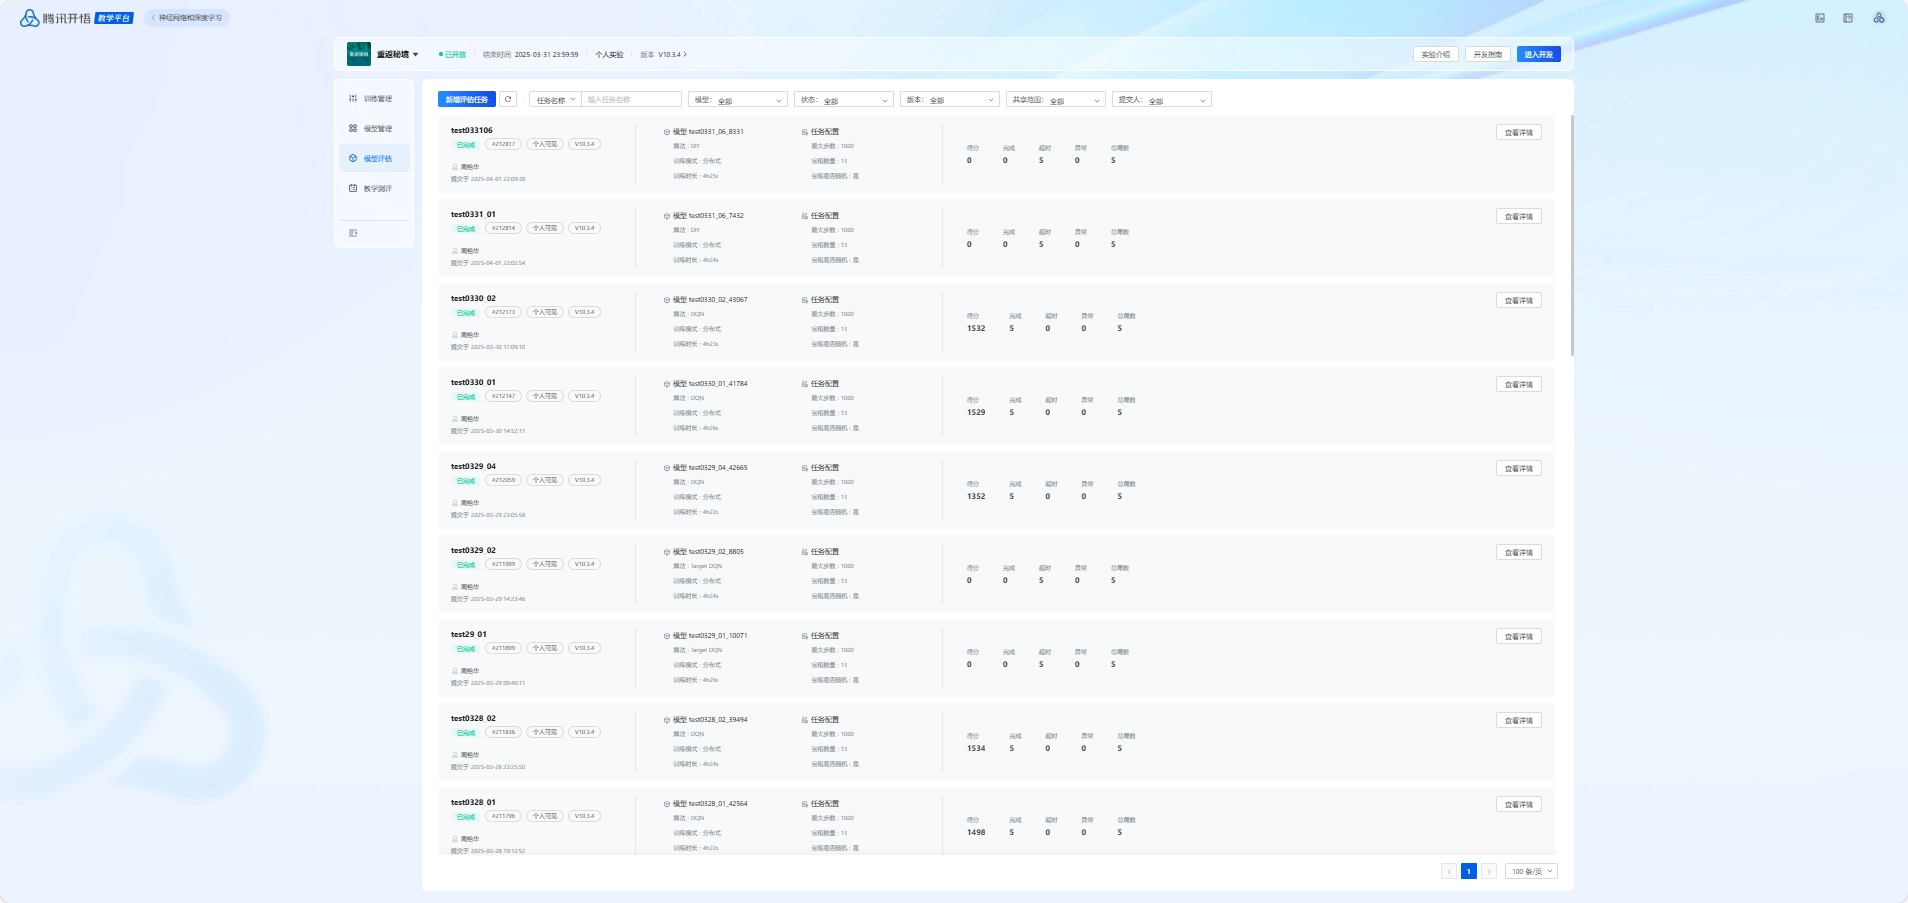
\includegraphics[width=0.8\linewidth]{pic/record-1.png}
    \caption{\zihao{-5} 实验记录1}
    \label{rec-1}
\end{figure}

\begin{figure}[H]
    \centering
    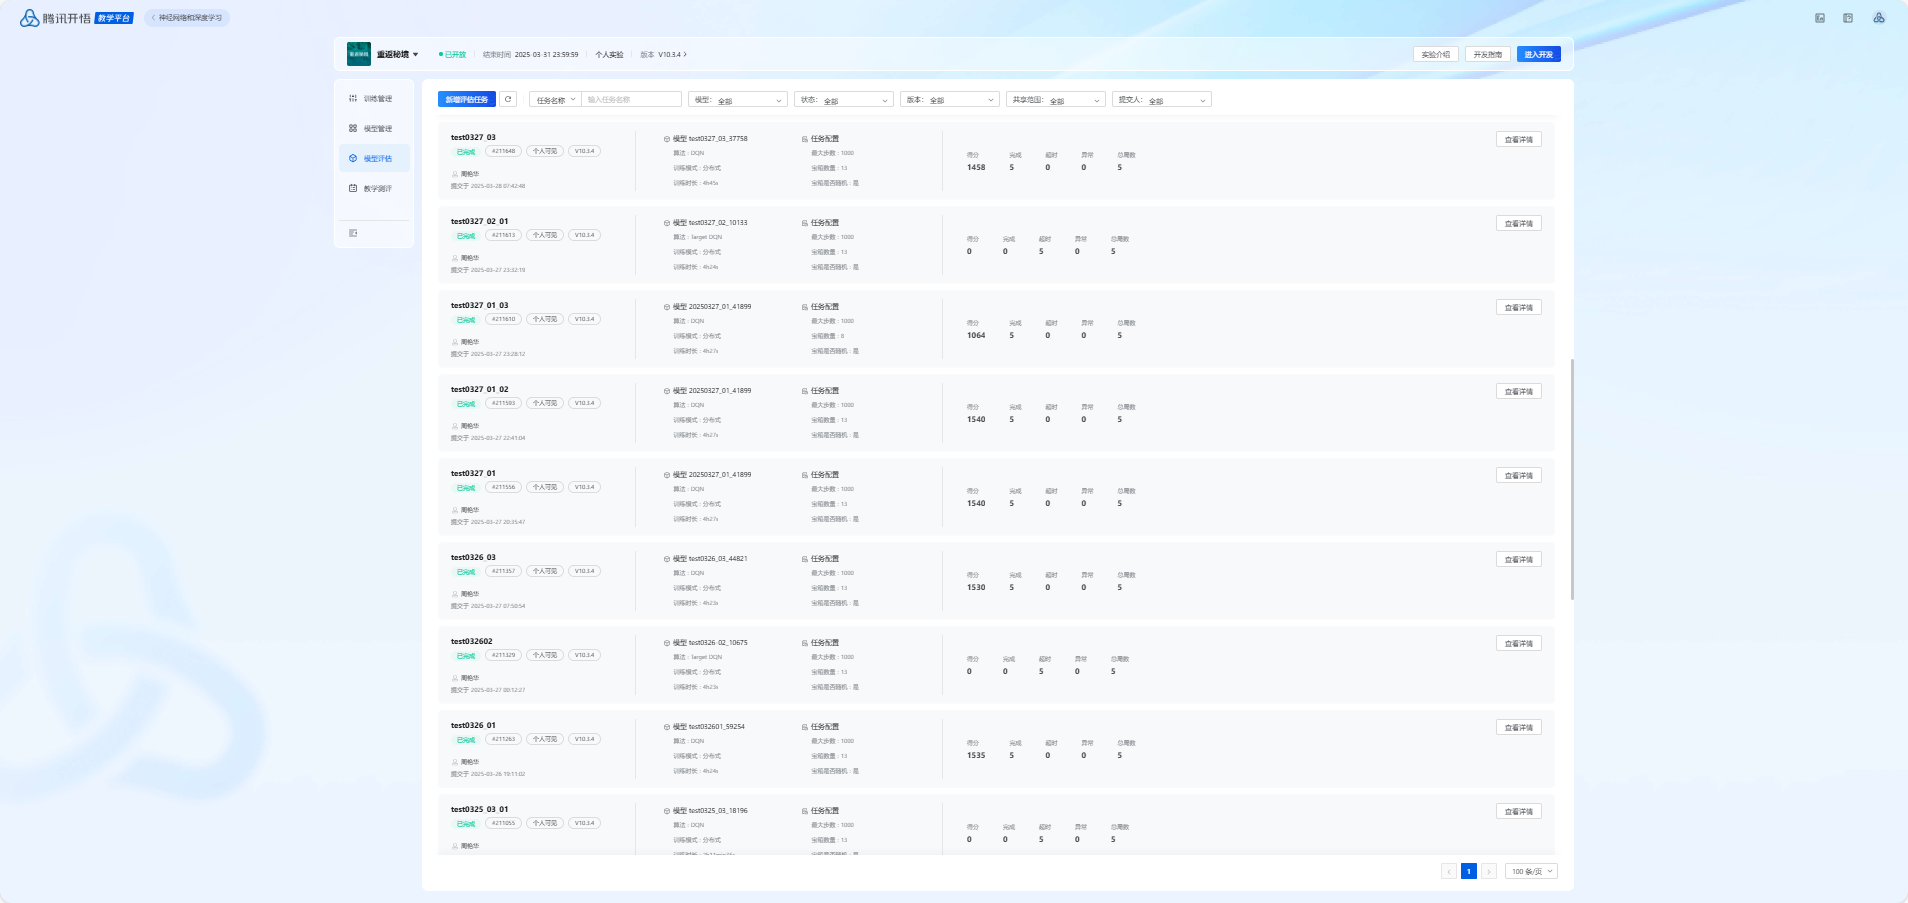
\includegraphics[width=0.8\linewidth]{pic/record-2.png}
    \caption{\zihao{-5} 实验记录2}
    \label{rec-2}
\end{figure}

\begin{figure}[H]
    \centering
    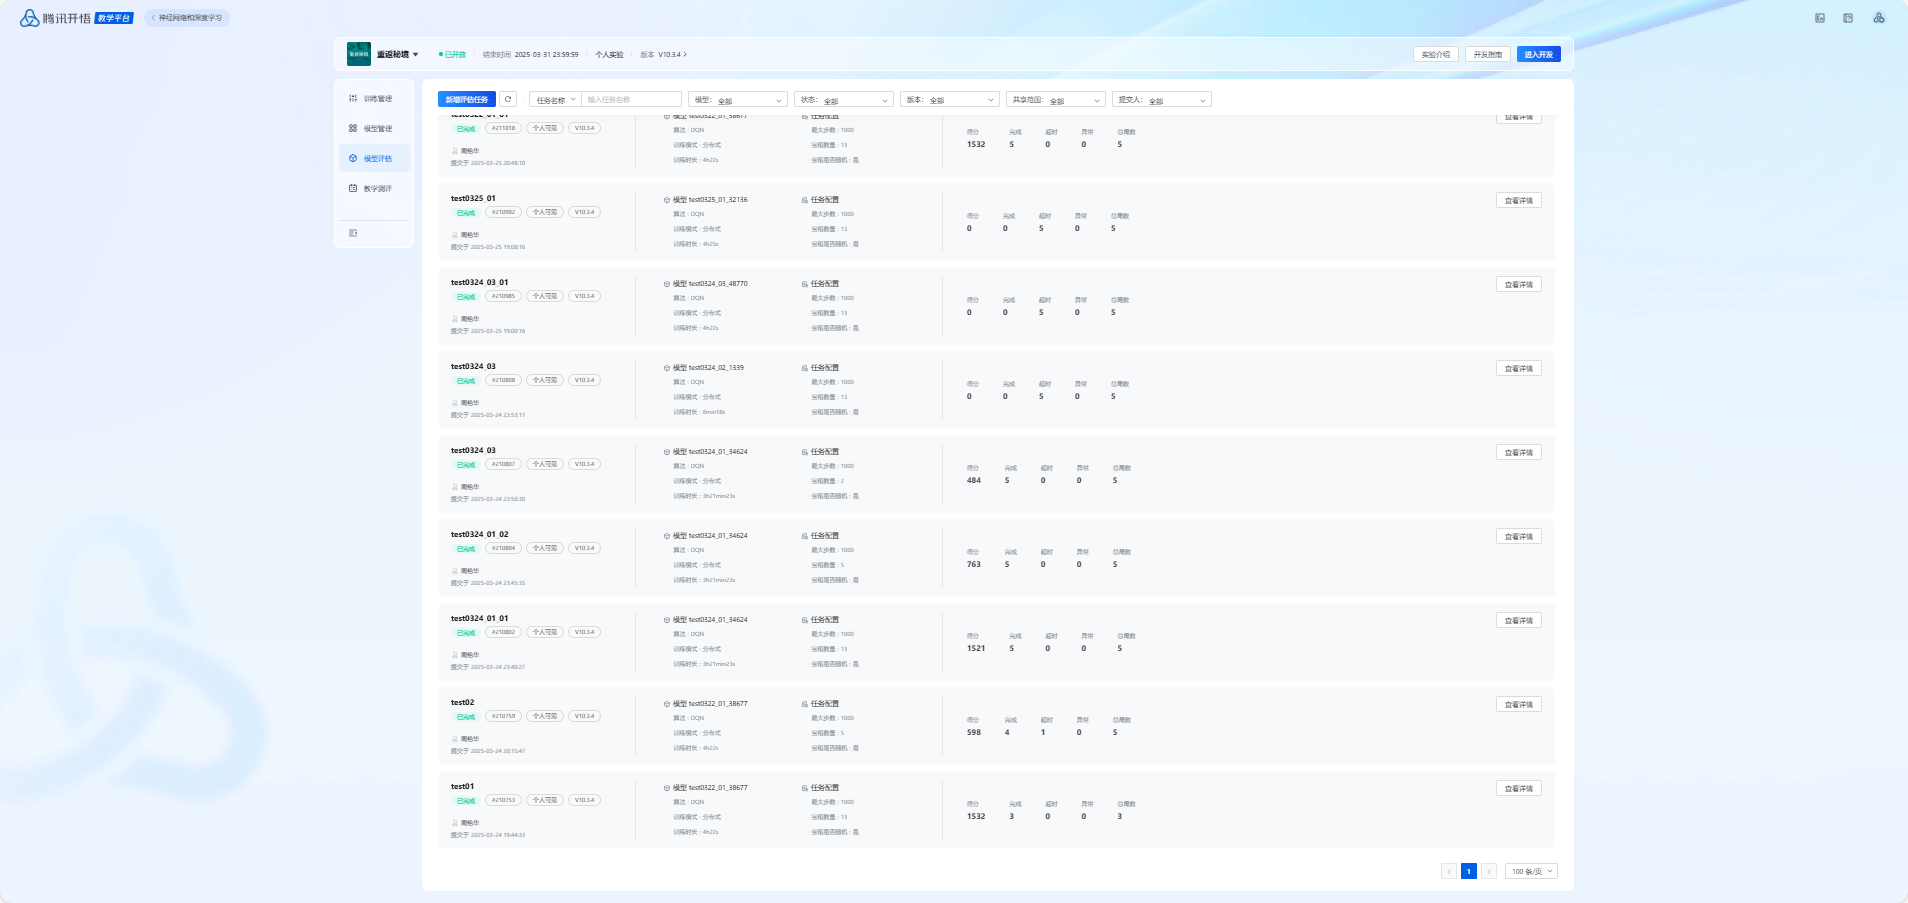
\includegraphics[width=0.8\linewidth]{pic/record-3.png}
    \caption{\zihao{-5} 实验记录3}
    \label{rec-3}
\end{figure}



\subsection{最佳分数}
多次实验得到的模型,在最大步数1000,宝箱数量13个的情况下,使用DNQ算法得到的最佳分数为1400.
\begin{figure}[H]
    \centering
    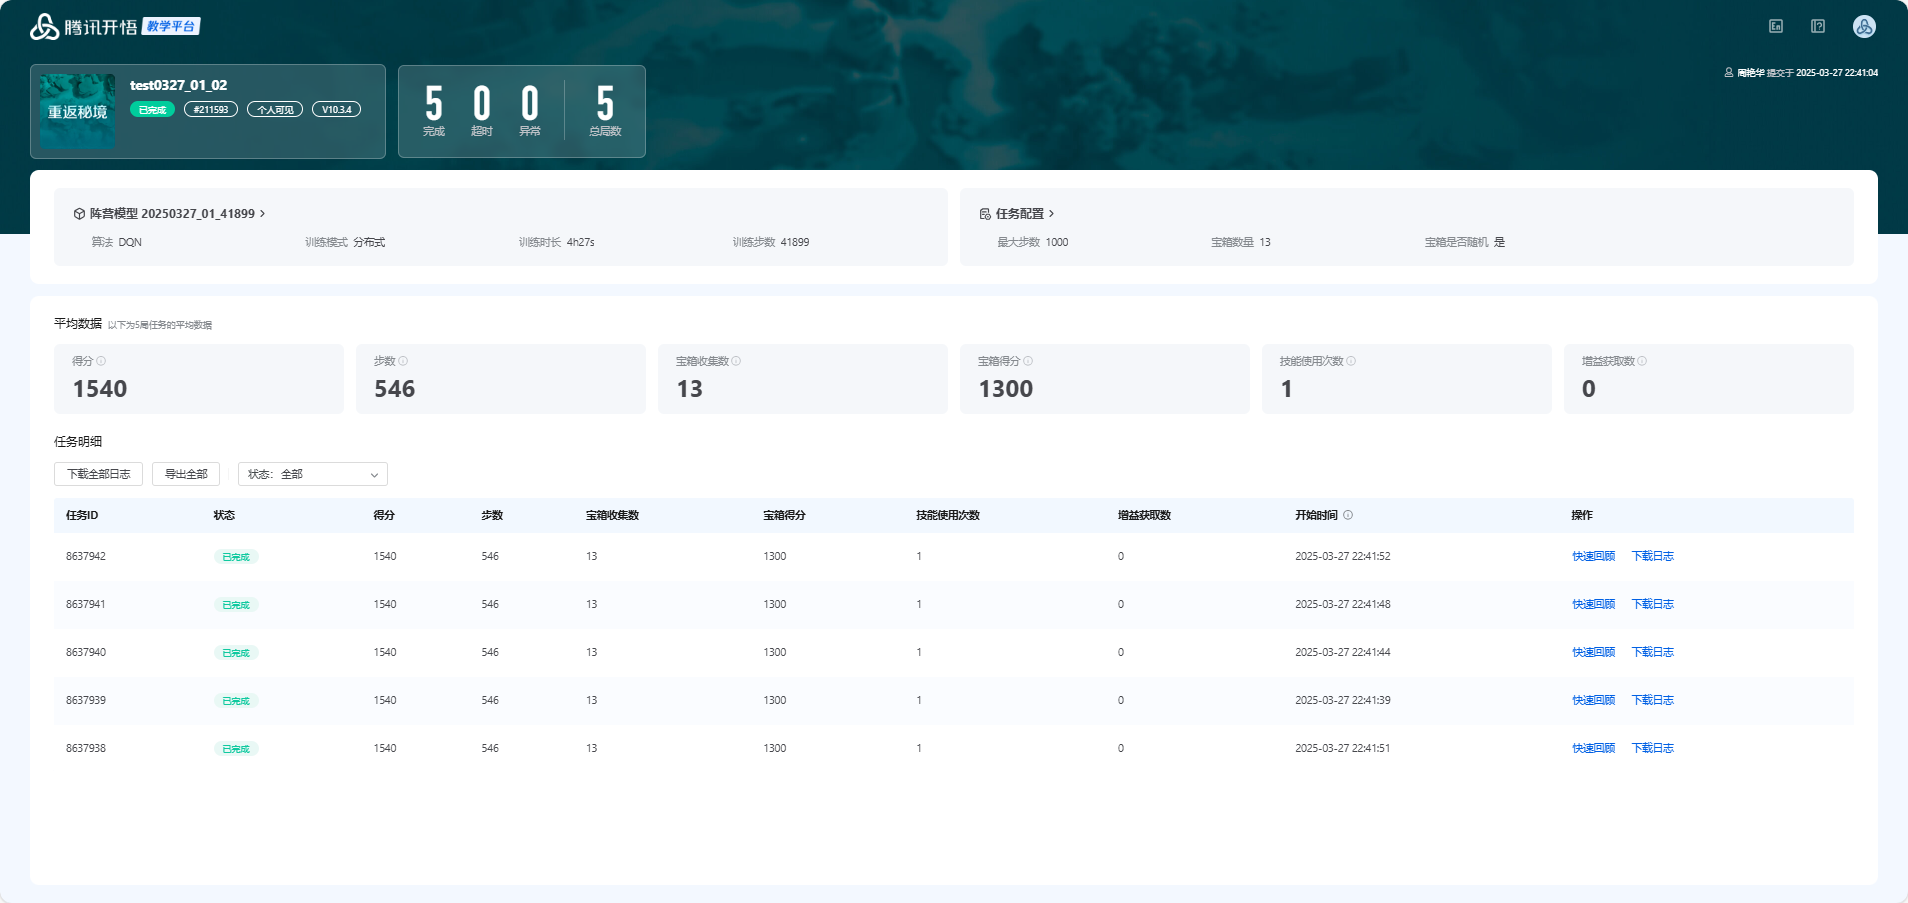
\includegraphics[width=0.8\linewidth]{pic/best-score.png}
    \caption{\zihao{-5} 最佳分数}
    \label{best-score}
\end{figure}
下图是最佳分数对应的路径概览。可以看出,如果能捡到加速,分数有可能能更高。(不过试了几次没有找到更高的)
\begin{figure}[H]
    \centering
    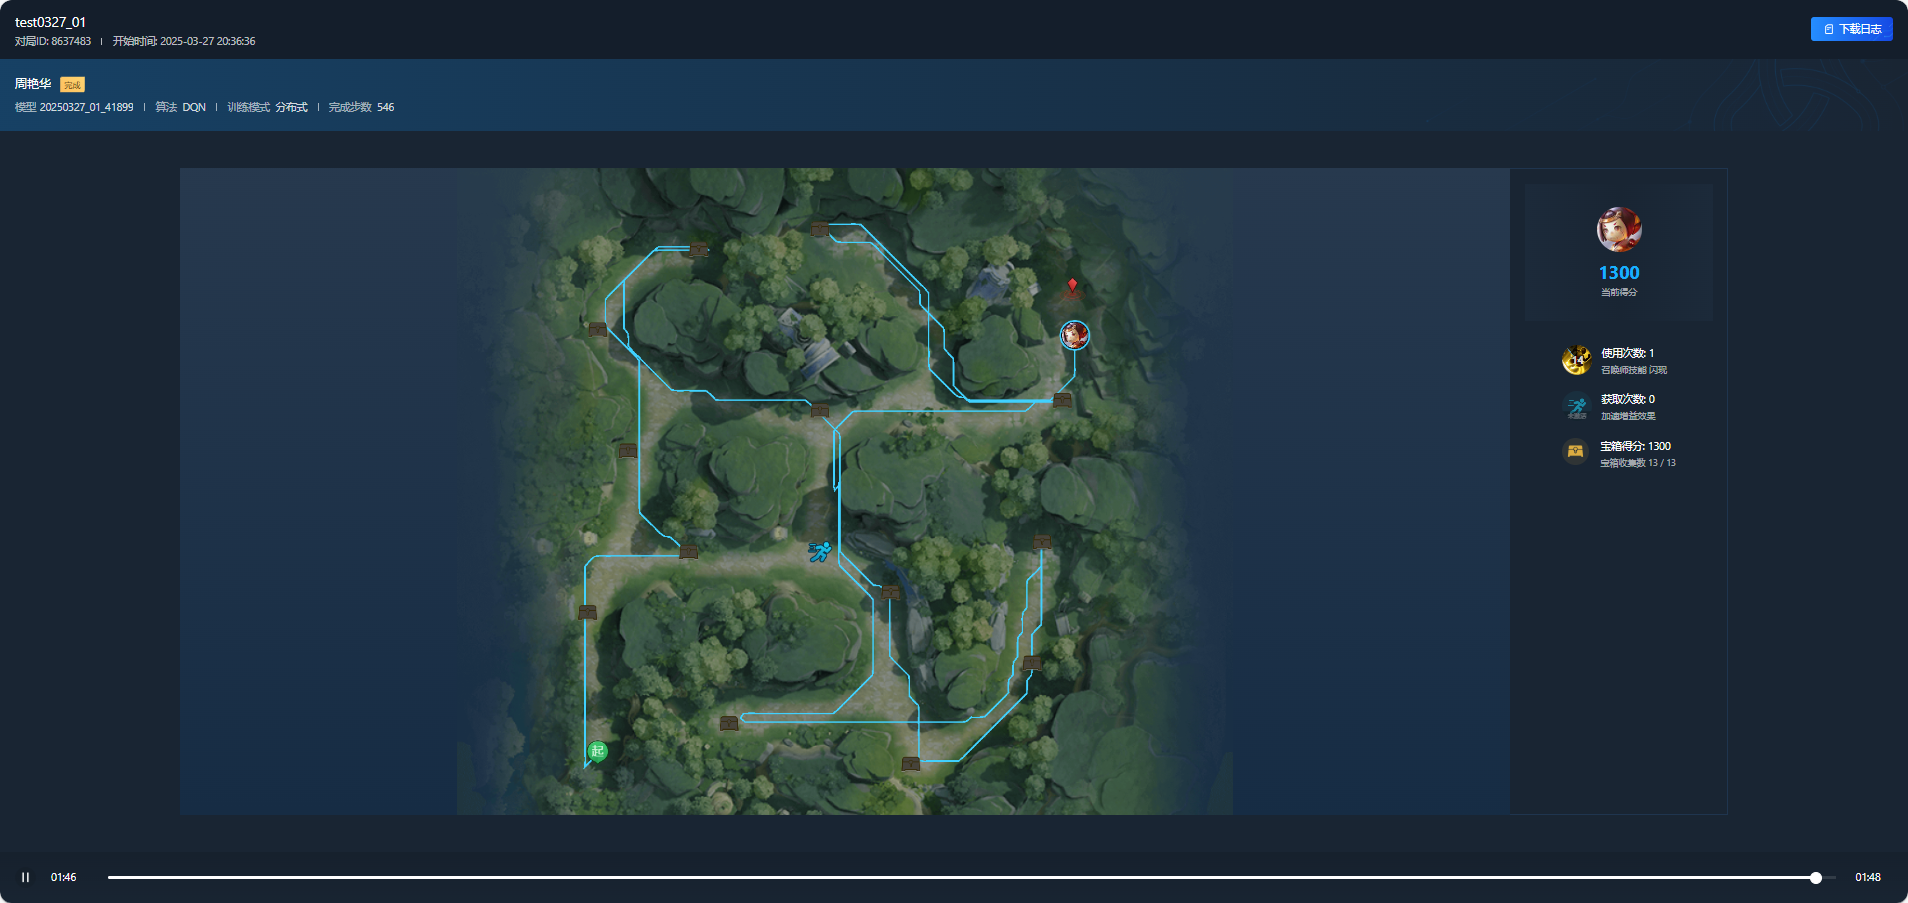
\includegraphics[width=0.8\linewidth]{pic/best-map.png}
    \caption{\zihao{-5} 路径概览}
    \label{path-overview}
\end{figure}